\documentclass[11pt,oneside,article]{memoir}
% !TEX root = ./CCC_Note.tex

\usepackage{amsmath}
\usepackage{amsthm}
\usepackage{amsfonts}
\usepackage{amssymb}
\usepackage{mathtools}
%\usepackage{datetime}
\usepackage[usenames,dvipsnames]{xcolor}
\usepackage[bookmarks=true,colorlinks=true, linkcolor=MidnightBlue, citecolor=cyan]{hyperref}
\usepackage[T1]{fontenc}
\usepackage[sc]{mathpazo}
\linespread{1.05}
\usepackage{mathrsfs}
\usepackage{euscript}
%\usepackage{MnSymbol}
\usepackage{paralist}
\usepackage{todonotes}
\usepackage{makecell}
\usepackage{booktabs}
\usepackage{tikz}
\usetikzlibrary{cd}
\usepackage{tensor}

\usetikzlibrary{decorations.markings,arrows.meta,calc,fit,quotes}
\hypersetup{final}

\DeclareMathOperator{\id}{id}
\DeclareMathOperator{\dom}{dom}
\DeclareMathOperator{\cod}{cod}
\DeclareMathOperator{\dvert}{Vert}
\DeclareMathOperator{\Lax}{Lax}
\DeclareMathOperator{\Hom}{Hom}
\DeclareMathOperator{\Ob}{Ob}
\DeclareMathOperator{\Tr}{Tr}


\theoremstyle{plain}
\newtheorem{theorem}{Theorem}[section]
\newtheorem*{theorem*}{Theorem}
\newtheorem{proposition}[theorem]{Proposition}
\newtheorem{corollary}[theorem]{Corollary}
\newtheorem{lemma}[theorem]{Lemma}
\newtheorem*{lemma*}{Lemma}

\theoremstyle{definition}
\newtheorem{definition}[theorem]{Definition}
\newtheorem{exercise}{Exercise}[section]

\theoremstyle{remark}
\newtheorem{example}[theorem]{Example}
\newtheorem{remark}[theorem]{Remark}

\newcommand{\prodb}{\mathbin{\Pi}}
\newcommand{\iso}{\cong}

\newcommand{\cat}[1]{\mathscr{#1}}
\newcommand{\Cat}[1]{\mathbf{#1}}
\newcommand{\fun}[1]{#1}
\newcommand{\Fun}[1]{\mathsf{#1}}
%\newcommand{\hom}{\mathrm{hom}}
\newcommand{\twocat}[1]{\mathcal{#1}}
\newcommand{\dblcat}[1]{\mathbb{#1}}
\newcommand{\Mon}{\Cat{Mon}}
\newcommand{\Prof}{\Cat{Prof}}
\newcommand{\MProf}{\Cat{MProf}}
\newcommand{\MonCat}{\Cat{MonCat}}
\newcommand{\SymMonCat}{\Cat{SymMonCat}}
\newcommand{\CompCat}{\Cat{CompCat}}
\newcommand{\TrCat}{\Cat{TrCat}}
\newcommand{\Set}{\Cat{Set}}
\newcommand{\Int}{\Fun{Int}}

\newcommand{\op}[1]{{#1}^{\text{op}}}
\newcommand{\vop}[1]{{#1}^{\text{vop}}}
\newcommand{\hop}[1]{{#1}^{\text{hop}}}

\newcommand{\Alg}{\mathrm{Alg}}
\newcommand{\Coalg}{\mathrm{Coalg}}
\newcommand{\RAlg}[1][]{\mathbb{R}_{#1}\text{-}\Alg}
\newcommand{\LCoalg}[1][]{\mathbb{L}_{#1}\text{-}\Coalg}
\newcommand{\LCoalgA}{\mathbb{L}_1\text{-}\Coalg}
\newcommand{\LCoalgB}{\mathbb{L}_2\text{-}\Coalg}

\newcommand{\twocell}[3][]{\arrow[draw=none,to path={(dom#2.center)--(cod#2.center)\tikztonodes}]{}[anchor=center,#1]{\Downarrow #3}}
\newcommand{\twocellalt}[3][]{\arrow[draw=none,to path={(dom#2.center)--(cod#2.center)\tikztonodes}]{}[anchor=center,#1]{#3}}
\newcommand{\twocellA}[2][]{\twocell[#1]{A}{#2}}
\newcommand{\twocellB}[2][]{\twocell[#1]{B}{#2}}
\newcommand{\twocellC}[2][]{\twocell[#1]{C}{#2}}
\newcommand{\twocellD}[2][]{\twocell[#1]{D}{#2}}
\newcommand{\twocellE}[2][]{\twocell[#1]{E}{#2}}
\newcommand{\twocellF}[2][]{\twocell[#1]{F}{#2}}



\tikzcdset{
	arrow style=tikz,
	diagrams={>={Classical TikZ Rightarrow[angle=63:4pt, line width=.6pt]}},
	arrows={semithick}
}

\tikzset{tick/.style={postaction={decorate,decoration={markings,mark=at position 0.5 with {\draw[-] (0,.4ex) -- (0,-.4ex);}}}}}
\tikzset{dom/.style={append after command={coordinate[alias=dom#1]}},
		domA/.style={dom=A}, domB/.style={dom=B},
		domC/.style={dom=C}, domD/.style={dom=D},
		domE/.style={dom=E}, domF/.style={dom=F}}
\tikzset{cod/.style={append after command={coordinate[alias=cod#1]}},
		codA/.style={cod=A}, codB/.style={cod=B},
		codC/.style={cod=C}, codD/.style={cod=D},
		codE/.style={cod=E}, codF/.style={cod=F}}


\tikzset{
	%label/.style={font=\everymath\expandafter{\the\everymath\scriptstyle}},
	wiring diagram/.style={
		every to/.style={out=0,in=180,draw},
		label/.style={
			font=\everymath\expandafter{\the\everymath\scriptstyle},
			inner sep=0pt,
			node distance=2pt and -2pt},
		semithick,
		node distance=1 and 1,
		decoration={markings, mark=at position .5 with {\arrow{stealth};}},
		ar/.style={postaction={decorate}},
		execute at begin picture={\tikzset{
			x=\bbx, y=\bby,
			every fit/.style={inner xsep=\bbx, inner ysep=\bby}}}
		},
	bbx/.store in=\bbx,
	bbx = 1.5cm,
	bby/.store in=\bby,
	bby = 1.75ex,
	bb port sep/.store in=\bbportsep,
	bb port sep=2,
	% bb wire sep/.store in=\bbwiresep,
	% bb wire sep=1.75ex,
	bb port length/.store in=\bbportlen,
	bb port length=4pt,
	bb min width/.store in=\bbminwidth,
	bb min width=1cm,
	bb rounded corners/.store in=\bbcorners,
	bb rounded corners=2pt,
	bb small/.style={bb port sep=1, bb port length=2.5pt, bbx=.4cm, bb min width=.4cm, bby=.7ex},
	bb/.code 2 args={
		\pgfmathsetlengthmacro{\bbheight}{\bbportsep * (max(#1,#2)+1) * \bby}
		\pgfkeysalso{draw,minimum height=\bbheight,minimum width=\bbminwidth,outer sep=0pt,
			rounded corners=\bbcorners,thick,
			prefix after command={\pgfextra{\let\fixname\tikzlastnode}},
			append after command={\pgfextra{\draw
				\ifnum #1=0{} \else foreach \i in {1,...,#1} {
					($(\fixname.north west)!{\i/(#1+1)}!(\fixname.south west)$) +(-\bbportlen,0) coordinate (\fixname_in\i) -- +(\bbportlen,0) coordinate (\fixname_in\i')}\fi
				\ifnum #2=0{} \else foreach \i in {1,...,#2} {
					($(\fixname.north east)!{\i/(#2+1)}!(\fixname.south east)$) +(-\bbportlen,0) coordinate (\fixname_out\i') -- +(\bbportlen,0) coordinate (\fixname_out\i)}\fi;
			}}}
	},
	bb name/.style={append after command={\pgfextra{\node[anchor=north] at (\fixname.north) {#1};}}}
}

\usetikzlibrary{arrows,calc,chains,matrix,positioning,scopes,snakes}


\newcommand{\vinp}[1]{\overline{\inp{#1}}}
\newcommand{\voutp}[1]{\overline{\outp{#1}}}
%\newcommand{\inp}[1]{#1^{\textnormal{in}}}
%\newcommand{\outp}[1]{#1^{\textnormal{out}}}
\newcommand{\inp}[1]{#1^-}
\newcommand{\outp}[1]{#1^+}

% \def\bhline{\Xhline{2\arrayrulewidth}}
% \def\bbhline{\Xhline{2.5\arrayrulewidth}}
\def\alg{{\text \textendash}\Cat{Alg}}
\def\XCat{\textnormal{$\Cat{X}$-$\Cat{Cat}$}}
\def\To{\xrightarrow}
\def\ul{\underline}
\def\List{\textnormal{List}}
\def\SList{\textnormal{SList}}
\def\SSList{\textnormal{SSList}}

\newcommand{\erase}[1]{{}}
\def\NN{\mathbb{N}}
\def\ss{\subseteq}
\def\boo{{\Ob\iso}}
\newcommand{\bo}{\mathsf{bo}}
\newcommand{\ff}{\mathsf{ff}}


\settrims{0pt}{0pt} % page and stock same size
%\setlxvchars %calculate line length such that there are about 65 characters per line in \normalfont
\settypeblocksize{*}{35pc}{*} % {height}{width}{ratio}
%\settypeblocksize{*}{39pc}{*} % {height}{width}{ratio}
\setlrmargins{*}{*}{1} % {spine}{edge}{ratio}
%\setulmargins{*}{*}{1} % {upper}{lower}{ratio}, hight of typeblock fixed
\setulmarginsandblock{1in}{1in}{*} % height of typeblock computed
\setheadfoot{\onelineskip}{2\onelineskip} % {headheight}{footskip}
\setheaderspaces{*}{1.5\onelineskip}{*} % {headdrop}{headsep}{ratio}
\checkandfixthelayout

\makeatletter
\def\blfootnote{\gdef\@thefnmark{}\@footnotetext}
\makeatother

\setcounter{tocdepth}{1}
\setcounter{secnumdepth}{2}
\pagestyle{ruled}
\renewcommand*{\chaptitlefont}{\bfseries\Large}
\setsecheadstyle{\bfseries\large\raggedright}
\setsubsecheadstyle{\bfseries\raggedright}

\renewcommand{\LabSet}{\mathcal{L}}

\title{Intuition/Talk on String diagrams for traced and compact categories are oriented 1-cobordisms}
\author{David I. Spivak, Patrick Schultz, Dylan Rupel}


\date{\vspace{-3ex}}

\begin{document}
\firmlists*

\maketitle


\begin{abstract}
  We will present an alternate conception of string diagrams as labeled 1-dimensional oriented cobordisms, the operad of which we denote by $\LCob{\LabSet}$, where $\LabSet$ is the set of string labels. The axioms of traced (symmetric monoidal) categories are fully encoded by $\LCob{\LabSet}$ in the sense that there is an equivalence between $\LCob{\LabSet}$-algebras, for varying $\LabSet$, and traced categories with varying object set. The same holds for compact (closed) categories, the difference being in terms of variance in $\LabSet$. Time permitting, we will give a characterization of the 2-category of traced categories solely in terms of those of monoidal and compact categories, without any reference to the usual structures or axioms of traced categories. 
\end{abstract}

\paragraph{Idea: operads can classify string diagram styles}
\begin{equation*}
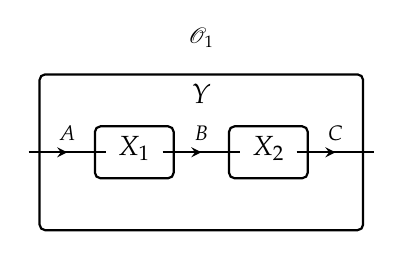
\begin{tikzpicture}[wiring diagram, bbx=1em, bby=1ex]
 \node[bb={1}{1},bb name=$X_1$] (X1) {};
 \node[bb={1}{1},right =2 of X1, bb name=$X_2$] (X2) {};
 \node[bb={1}{1}, fit={($(X1.north west)+(-1,3)$) ($(X1.south)+(0,-3)$) ($(X2.east)+(1,0)$)}, bb name = $Y$] (Y) {};
%
 \draw[ar] (Y_in1') to (X1_in1);
 \draw[ar] (X1_out1) to (X2_in1);
 \draw[ar] (X2_out1) to (Y_out1');
 \draw[label] 
	node at ($(Y_in1')!.5!(X1_in1)+(0,7pt)$)  {$A$}
	node at ($(X1_out1)!.5!(X2_in1)+(0,7pt)$)   {$B$}
	node at ($(X2_out1)!.5!(Y_out1')+(0,7pt)$)  {$C$}
	node[above=2] at (Y.north) {$\cat{O}_1$};
\end{tikzpicture}
\qquad
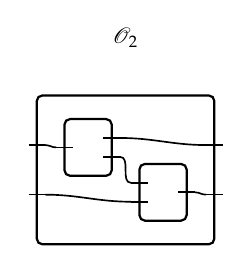
\begin{tikzpicture}[wiring diagram, bb min width =.6cm, bb port sep =.8, bby=.3cm, bbx=1em,bb port length=3pt]
  \node[bb={1}{2}] (X1) {};
  \node[bb={2}{1}, below right=-.5 and 1 of X1] (X2) {};
  \node[bb={2}{2}, fit=(X1) (X2)] (Y) {};
  \draw (Y_in1') to (X1_in1);
  \draw (Y_in2') to (X2_in2);
  \draw (X1_out1) to (Y_out1');
  \draw (X1_out2) to (X2_in1);
  \draw (X2_out1) to (Y_out2');
  \draw[label] node[above=2] at (Y.north) {$\cat{O}_2$};
\end{tikzpicture}
\qquad
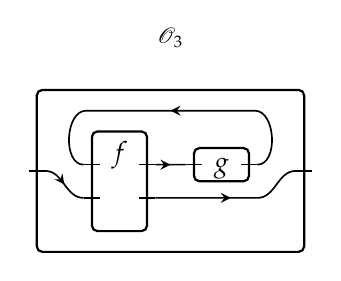
\begin{tikzpicture}[wiring diagram, bb min width =.7cm, bby=1.6ex, bbx=.7cm,bb port length=3pt] 
  \node[bb port sep=1.6, bb={2}{2}, bb name=$f$] (X1) {};
  \node[bb port sep=.8,bb={1}{1}, right=.7 of X1_out1, bb name=$g$] (X2) {};
  \node[bb={1}{1}, fit={(X1) (X2) ($(X1.north)+(0,1)$)}] (Y) {};
  \draw[ar] (Y_in1') to (X1_in2);
  \draw[ar,pos=.8] (X1_out1) to (X2_in1);
  \draw[ar] let \p1=(X2.south east), \n1={\y1-.8*\bby}, \n2=\bbportlen in
          (X1_out2) -- (\x1+\n2,\n1) to (Y_out1');
  \draw[ar] let \p1=(X2.north east), \p2=(X1.north west), \n1={\y2+\bby}, \n2=\bbportlen in
          (X2_out1) to[in=0] (\x1+.7*\n2,\n1) -- (\x2-.7*\n2,\n1) to[out=180] (X1_in1);
   \draw[label] node[above=2] at (Y.north) {$\cat{O}_3$};
\end{tikzpicture}
\end{equation*}
for categories, monoidal categories, traced monoidal categories, etc.
Then 
\[\Lax(\cat{O},\Set) = \text{categories of sort $\cat{O}$. "Doctrine"}\]
Here $\Set$ is acting as an enriching category.

\paragraph{Traced monoidal categories.} Joyal, Street, Verity defined these. [All monoidal cats today are symmetric.] A \emph{traced category} is a monoidal category $(\cat{C},\otimes,I)$ + ... For all $X,Y,U\in\cat{C}$ a function 
\[\Tr^U_{X,Y}\colon\Hom(X\otimes U,Y\otimes U)\to\Hom(X,Y)\]
satisfying certain axioms, e.g.
\begin{center}
	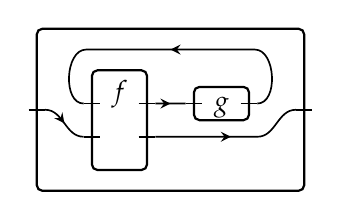
\begin{tikzpicture}[wiring diagram, bb min width =.7cm, bby=1.6ex, bbx=.7cm,bb port length=3pt,baseline=(current bounding box.center)] 
		\node[bb port sep=1.6, bb={2}{2}, bb name=$f$] (X1) {};
		\node[bb port sep=.8,bb={1}{1}, right=.7 of X1_out1, bb name=$g$] (X2) {};
		\node[bb={1}{1}, fit={(X1) (X2) ($(X1.north)+(0,1)$)}] (Y) {};
		\draw[ar] (Y_in1') to (X1_in2);
		\draw[ar,pos=.8] (X1_out1) to (X2_in1);
		\draw[ar] let \p1=(X2.south east), \n1={\y1-.8*\bby}, \n2=\bbportlen in 
			(X1_out2) -- (\x1+\n2,\n1) to (Y_out1');
		\draw[ar] let \p1=(X2.north east), \p2=(X1.north west), \n1={\y2+\bby}, \n2=\bbportlen in
			(X2_out1) to[in=0] (\x1+.7*\n2,\n1) -- (\x2-.7*\n2,\n1) to[out=180] (X1_in1);
	\end{tikzpicture}
\quad
=
\quad
	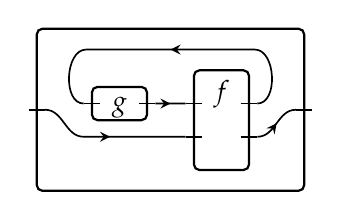
\begin{tikzpicture}[wiring diagram, bb min width =.7cm, bby=1.6ex, bbx=.7cm,bb port length=3pt,baseline=(current bounding box.center)] 
		\node[bb port sep=1.6, bb={2}{2}, bb name=$f$] (X1) {};
		\node[bb port sep=.8,bb={1}{1}, left=.7 of X1_in1, bb name=$g$] (X2) {};
		\node[bb={1}{1}, fit={(X2) (X1) ($(X1.north)+(0,1)$)}] (Y) {};
		\draw[ar] (X1_out2) to (Y_out1');
		\draw[ar,pos=.8] (X2_out1) to (X1_in1);
		\draw[ar] let \p1=(X2.south west), \n1={\y1-.8*\bby}, \n2=\bbportlen in
			(Y_in1') to (\x1-\n2,\n1) -- (X1_in2);
		\draw[ar] let \p1=(X2.north west), \p2=(X1.north east), \n1={\y2+\bby}, \n2=\bbportlen in
			(X1_out1) to[in=0] (\x2+.7*\n2,\n1) -- (\x1-.7*\n2,\n1) to[out=180] (X2_in1);
	\end{tikzpicture}
\end{center}
\[\Tr\big((g\otimes\id_Y)\circ f\big)=\Tr\big(f\circ(g\otimes\id_X)\big).\]
They also defined 2-adjunction
\[\Int\colon\TTrCat\leftrightarrows\CCompCat\cocolon U\]
Two more facts:
\begin{itemize}
\item The unit $T\to U\Int(T)$ is fully faithful for all traced $T$.
\item Any monoidal M, compact $C$, and fully faithful $M\hookrightarrow C$ induces a unique trace structure on $M$ for which the map is traced.
\end{itemize}
\paragraph{(bo,ff) factorization system} The 2-categories $\MMonCat$, $\TTrCat$, and $\CCompCat$ have (compatible) bo-ff orthogonal factorization systems.
\paragraph{Traceless characterization} The 2-cat $\TTrCat$ of traced categories is equivalent to $\TrFrObCat$, whose objects are
\[\Ob(\TrFrObCat)=\big\{(\LabSet,C,F)\mid \LabSet\in\Set, C\in\CompCat, F\colon\text{FreeMonCat}(\LabSet)\to C\big\}\]
Morphisms are $\LabSet\to\LabSet'$ and $C\to C'$ making the diagram commute. The equivalence is given by factoring the maps $\text{FreeMonCat}(\LabSet)\to C$ as bo-ff.

\paragraph{$\Cob$ is the operad for traced and compact categories.}
\[
\parbox{2in}{
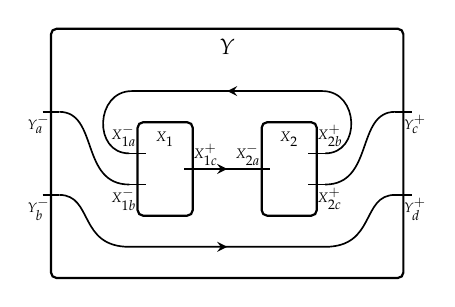
\begin{tikzpicture}[wiring diagram, bb min width =.7cm, bby=1.2ex, bbx=1.1cm,bb port length=3pt,
	label/.append style={node distance=1pt and -3pt}] 
  \node[bb={2}{1},, bb name={\tiny $X_1$}] (X1) {};
  \node[bb={1}{2}, right=.7 of X1_out1, bb name={\tiny $X_2$}] (X2) {};
  \node[bb={2}{2}, fit={(X1) (X2) ($(X1.south)-(0,3)$) ($(X1.north)+(0,5)$)}, bb name={\footnotesize$Y$}] (Y) {};
  \draw (Y_in1') to[in looseness=1.25] (X1_in2);
  \draw[ar,pos=.8] (X1_out1) to (X2_in1);
  \draw (X2_out2) to[out looseness=1.25] (Y_out1');
  \draw[ar] let \p1=(X1.south west), \p2=(X2.south east), \n1={\y2-2*\bby}, \n2=\bbportlen in
  	(Y_in2') to[in looseness=1.5] (\x1-\n2,\n1) -- (\x2+\n2,\n1) to[out looseness=1.5] (Y_out2');
  \draw[ar] let \p1=(X2.north east), \p2=(X1.north west), \n1={\y2+2*\bby}, \n2=\bbportlen in
   	(X2_out1) to[in=0, looseness=1.5] (\x1+.7*\n2,\n1) -- (\x2-.7*\n2,\n1) to[out=180, looseness=1.5] (X1_in1);
  \draw[label] 
        node[above left=2pt and -3pt of X1_in1] {\tiny$\inp{X}_{1a}$}
        node[below left=of X1_in2] {\tiny$\inp{X}_{1b}$}
        node[above right=of X1_out1] {\tiny$\outp{X}_{1c}$}
        node[above left=of X2_in1] {\tiny$\inp{X}_{2a}$}
        node[above right=2pt and -3pt of X2_out1] {\tiny$\outp{X}_{2b}$}
        node[below right=of X2_out2] {\tiny$\outp{X}_{2c}$}
        node[below left=of Y_in1] {\tiny$\inp{Y}_{a}$}
        node[below left=of Y_in2] {\tiny$\inp{Y}_{b}$}
        node[below right=of Y_out1] {\tiny$\outp{Y}_{c}$}
        node[below right=of Y_out2] {\tiny$\outp{Y}_{d}$}
        ;

\end{tikzpicture}
}
\qquad
\parbox{1.8in}{
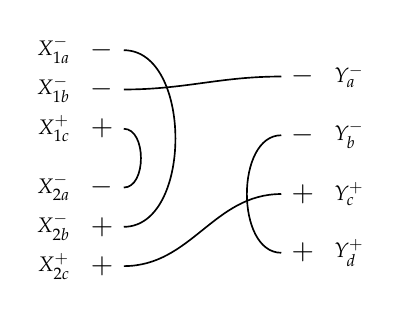
\begin{tikzpicture}[x=1cm,y=1ex,node distance=1 and 1,semithick,every label quotes/.style={font=\everymath\expandafter{\the\everymath\scriptstyle}},every to/.style={out=0,in=180},baseline=(current bounding box.center)]
  \node ["$\inp{X}_{1a}$" left] (X1a) {$-$};
  \node [below=0 of X1a, "$\inp{X}_{1b}$" left] (X1b) {$-$};
  \node [below=0 of X1b, "$\outp{X}_{1c}$" left] (X1c) {$+$};
  \node [below=1.5 of X1c, "$\inp{X}_{2a}$" left] (X2a) {$-$};
  \node [below=0 of X2a, "$\inp{X}_{2b}$" left] (X2b) {$+$};
  \node [below=0 of X2b, "$\outp{X}_{2c}$" left] (X2c) {$+$};
  \node [below right=-1 and 2 of X1a, "$\inp{Y}_a$" right] (Ya) {$-$};
  \node [below=1.5 of Ya, "$\inp{Y}_b$" right] (Yb) {$-$};
  \node [below=1.5 of Yb, "$\outp{Y}_c$" right] (Yc) {$+$};
  \node [below=1.5 of Yc, "$\outp{Y}_d$" right] (Yd) {$+$};
  \draw (X1a) to[in=0] (X2b);
  \draw (X1b) to (Ya);
  \draw (X1c) to[in=0] (X2a);
  \draw (X2c) to (Yc);
  \draw (Yb) to[out=180] (Yd);
\end{tikzpicture}
}
\]

\paragraph{Fully faithful $\MonCat\to\text{Oprd}$.} $\Cob$ as a monoidal category is sent to $\Cob$ as an operad. Since the functor is fully faithful, we can work either place. $\MonCat$ is more convenient, but $\text{Oprd}$ has better pictures.

\paragraph{Some results}
Let $\LabSet\in\Set$. Then we have an equivalence of categories
\[\Lax(\Cob/\LabSet,\Set)\cong\TrCat_{\LabSet}\]
where the latter is the 1-category of traced cats with object set free on $\LabSet$.

More generally, let $T$ be any traced category. Then we have an equivalence
\[\Lax(\Int(T),\Set)\cong\TrCat^{\bo}_{T/}\]
Similarly, let $C$ be any compact category. We have an equivalence
\begin{equation}\label{more_later}
\Lax(C,\Set)\cong\CompCat^{\bo}_{C/}
\end{equation}
But putting these together we get something a little funny.
\[\TrCat^{\bo}_{T/}\cong\Lax(\Int(T),\Set)\cong\CompCat^{\bo}_{Int(T)/}\]
Here's the idea. Given $T\onto T'$ we get $\Int(T)\onto\Int(T')$; that's one direction. For the other direction, given $\Int(T)\onto C'$, we factor its composite with the unit $T\to\Int(T)$:
\[
\begin{tikzcd}
T\ar[r]\ar[d,two heads]&\Int(T)\ar[d]\\
T'\ar[r,hook]&C'
\end{tikzcd}
\]
giving $T\onto T'$.
\begin{corollary}
Since $\Cob/\LabSet$ is the free compact category on $\LabSet\in\Set$, it follows that 
\[\TrCat_\LabSet\cong\Lax(\Cob/\LabSet,\Set)\cong\CompCat_{\LabSet}\]
\end{corollary}

Let's give intuition for \eqref{more_later}.
\begin{theorem}
\[\Lax(C,\Set)\cong\CompCat^{\bo}_{C/}\]
\end{theorem}
\begin{proof}[Proof intuition]
~\\
$\Leftarrow$: Suppose given $F\colon C\onto C'$. We construct $L_F\colon C\to\Set$ by
\[L_F(c)\coloneqq\Hom_{C'}(I,c)\]
where $c$ is an object or morphism of $C'$ and $I$ is the monoidal unit in $C'$. The lax structure is 
\[
L_F(c)\times L_F(c')=\Hom(I,c)\times\Hom(I,c')\To{\otimes}
\Hom(I\otimes I,c\otimes c')=L_F(c\otimes c').
\]
~\\
$\Rightarrow$: Suppose given $L\colon C\to\Set$. We want $F_L\colon C\onto C'$. Since its bijective on objects, we can put $\Ob(C)=\Ob(C')$, what about the morphisms of $C'$?
\[
\Hom_{C'}(c_1,c_2)=L(c_1^*\otimes c_2).
\]
Composition comes from the lax structure.
\end{proof}



\end{document}
